\documentclass[]{book}
\usepackage{lmodern}
\usepackage{amssymb,amsmath}
\usepackage{ifxetex,ifluatex}
\usepackage{fixltx2e} % provides \textsubscript
\ifnum 0\ifxetex 1\fi\ifluatex 1\fi=0 % if pdftex
  \usepackage[T1]{fontenc}
  \usepackage[utf8]{inputenc}
\else % if luatex or xelatex
  \ifxetex
    \usepackage{mathspec}
  \else
    \usepackage{fontspec}
  \fi
  \defaultfontfeatures{Ligatures=TeX,Scale=MatchLowercase}
\fi
% use upquote if available, for straight quotes in verbatim environments
\IfFileExists{upquote.sty}{\usepackage{upquote}}{}
% use microtype if available
\IfFileExists{microtype.sty}{%
\usepackage{microtype}
\UseMicrotypeSet[protrusion]{basicmath} % disable protrusion for tt fonts
}{}
\usepackage{hyperref}
\hypersetup{unicode=true,
            pdftitle={Indicateurs de la Biodiversité},
            pdfauthor={Andrew MacDonald},
            pdfborder={0 0 0},
            breaklinks=true}
\urlstyle{same}  % don't use monospace font for urls
\usepackage{natbib}
\bibliographystyle{apalike}
\usepackage{color}
\usepackage{fancyvrb}
\newcommand{\VerbBar}{|}
\newcommand{\VERB}{\Verb[commandchars=\\\{\}]}
\DefineVerbatimEnvironment{Highlighting}{Verbatim}{commandchars=\\\{\}}
% Add ',fontsize=\small' for more characters per line
\usepackage{framed}
\definecolor{shadecolor}{RGB}{248,248,248}
\newenvironment{Shaded}{\begin{snugshade}}{\end{snugshade}}
\newcommand{\AlertTok}[1]{\textcolor[rgb]{0.94,0.16,0.16}{#1}}
\newcommand{\AnnotationTok}[1]{\textcolor[rgb]{0.56,0.35,0.01}{\textbf{\textit{#1}}}}
\newcommand{\AttributeTok}[1]{\textcolor[rgb]{0.77,0.63,0.00}{#1}}
\newcommand{\BaseNTok}[1]{\textcolor[rgb]{0.00,0.00,0.81}{#1}}
\newcommand{\BuiltInTok}[1]{#1}
\newcommand{\CharTok}[1]{\textcolor[rgb]{0.31,0.60,0.02}{#1}}
\newcommand{\CommentTok}[1]{\textcolor[rgb]{0.56,0.35,0.01}{\textit{#1}}}
\newcommand{\CommentVarTok}[1]{\textcolor[rgb]{0.56,0.35,0.01}{\textbf{\textit{#1}}}}
\newcommand{\ConstantTok}[1]{\textcolor[rgb]{0.00,0.00,0.00}{#1}}
\newcommand{\ControlFlowTok}[1]{\textcolor[rgb]{0.13,0.29,0.53}{\textbf{#1}}}
\newcommand{\DataTypeTok}[1]{\textcolor[rgb]{0.13,0.29,0.53}{#1}}
\newcommand{\DecValTok}[1]{\textcolor[rgb]{0.00,0.00,0.81}{#1}}
\newcommand{\DocumentationTok}[1]{\textcolor[rgb]{0.56,0.35,0.01}{\textbf{\textit{#1}}}}
\newcommand{\ErrorTok}[1]{\textcolor[rgb]{0.64,0.00,0.00}{\textbf{#1}}}
\newcommand{\ExtensionTok}[1]{#1}
\newcommand{\FloatTok}[1]{\textcolor[rgb]{0.00,0.00,0.81}{#1}}
\newcommand{\FunctionTok}[1]{\textcolor[rgb]{0.00,0.00,0.00}{#1}}
\newcommand{\ImportTok}[1]{#1}
\newcommand{\InformationTok}[1]{\textcolor[rgb]{0.56,0.35,0.01}{\textbf{\textit{#1}}}}
\newcommand{\KeywordTok}[1]{\textcolor[rgb]{0.13,0.29,0.53}{\textbf{#1}}}
\newcommand{\NormalTok}[1]{#1}
\newcommand{\OperatorTok}[1]{\textcolor[rgb]{0.81,0.36,0.00}{\textbf{#1}}}
\newcommand{\OtherTok}[1]{\textcolor[rgb]{0.56,0.35,0.01}{#1}}
\newcommand{\PreprocessorTok}[1]{\textcolor[rgb]{0.56,0.35,0.01}{\textit{#1}}}
\newcommand{\RegionMarkerTok}[1]{#1}
\newcommand{\SpecialCharTok}[1]{\textcolor[rgb]{0.00,0.00,0.00}{#1}}
\newcommand{\SpecialStringTok}[1]{\textcolor[rgb]{0.31,0.60,0.02}{#1}}
\newcommand{\StringTok}[1]{\textcolor[rgb]{0.31,0.60,0.02}{#1}}
\newcommand{\VariableTok}[1]{\textcolor[rgb]{0.00,0.00,0.00}{#1}}
\newcommand{\VerbatimStringTok}[1]{\textcolor[rgb]{0.31,0.60,0.02}{#1}}
\newcommand{\WarningTok}[1]{\textcolor[rgb]{0.56,0.35,0.01}{\textbf{\textit{#1}}}}
\usepackage{longtable,booktabs}
\usepackage{graphicx,grffile}
\makeatletter
\def\maxwidth{\ifdim\Gin@nat@width>\linewidth\linewidth\else\Gin@nat@width\fi}
\def\maxheight{\ifdim\Gin@nat@height>\textheight\textheight\else\Gin@nat@height\fi}
\makeatother
% Scale images if necessary, so that they will not overflow the page
% margins by default, and it is still possible to overwrite the defaults
% using explicit options in \includegraphics[width, height, ...]{}
\setkeys{Gin}{width=\maxwidth,height=\maxheight,keepaspectratio}
\IfFileExists{parskip.sty}{%
\usepackage{parskip}
}{% else
\setlength{\parindent}{0pt}
\setlength{\parskip}{6pt plus 2pt minus 1pt}
}
\setlength{\emergencystretch}{3em}  % prevent overfull lines
\providecommand{\tightlist}{%
  \setlength{\itemsep}{0pt}\setlength{\parskip}{0pt}}
\setcounter{secnumdepth}{5}
% Redefines (sub)paragraphs to behave more like sections
\ifx\paragraph\undefined\else
\let\oldparagraph\paragraph
\renewcommand{\paragraph}[1]{\oldparagraph{#1}\mbox{}}
\fi
\ifx\subparagraph\undefined\else
\let\oldsubparagraph\subparagraph
\renewcommand{\subparagraph}[1]{\oldsubparagraph{#1}\mbox{}}
\fi

%%% Use protect on footnotes to avoid problems with footnotes in titles
\let\rmarkdownfootnote\footnote%
\def\footnote{\protect\rmarkdownfootnote}

%%% Change title format to be more compact
\usepackage{titling}

% Create subtitle command for use in maketitle
\providecommand{\subtitle}[1]{
  \posttitle{
    \begin{center}\large#1\end{center}
    }
}

\setlength{\droptitle}{-2em}

  \title{Indicateurs de la Biodiversité}
    \pretitle{\vspace{\droptitle}\centering\huge}
  \posttitle{\par}
    \author{Andrew MacDonald}
    \preauthor{\centering\large\emph}
  \postauthor{\par}
      \predate{\centering\large\emph}
  \postdate{\par}
    \date{2020-06-19}

\usepackage{booktabs}

\begin{document}
\maketitle

{
\setcounter{tocdepth}{1}
\tableofcontents
}
\hypertarget{dependencies}{%
\chapter{Dependencies}\label{dependencies}}

\begin{Shaded}
\begin{Highlighting}[]
\KeywordTok{library}\NormalTok{(rcoleo)}
\KeywordTok{library}\NormalTok{(tidyverse)}
\KeywordTok{library}\NormalTok{(lubridate)}
\end{Highlighting}
\end{Shaded}

\hypertarget{dl}{%
\chapter{Download data}\label{dl}}

The only point here is to demonstrate the workflow for downloading data

\begin{Shaded}
\begin{Highlighting}[]
\CommentTok{# On retire les cellules (classe sf) depuis l'API}
\NormalTok{cells <-}\StringTok{ }\NormalTok{rcoleo}\OperatorTok{::}\KeywordTok{sf_cells}\NormalTok{()}
\NormalTok{obs <-}\StringTok{ }\NormalTok{rcoleo}\OperatorTok{::}\KeywordTok{get_obs}\NormalTok{()}
\NormalTok{sites_dl <-}\StringTok{ }\NormalTok{rcoleo}\OperatorTok{::}\KeywordTok{sf_sites}\NormalTok{()}

\CommentTok{# until there is a better way to obtain the data and parse the result (perhaps}
\CommentTok{# in the form of a convenience function in rcoleo) we do this:}

\NormalTok{obs_df <-}\StringTok{ }\NormalTok{obs[[}\DecValTok{1}\NormalTok{]] }\OperatorTok\StringTok{ }\KeywordTok{map}\NormalTok{(}\StringTok{"body"}\NormalTok{) }\OperatorTok\StringTok{ }\KeywordTok{map_df}\NormalTok{(}\OperatorTok{~}\StringTok{ }\KeywordTok{select}\NormalTok{(.x, }\OperatorTok{-}\NormalTok{closed_at))}

\NormalTok{all_obs <-}\StringTok{ }\NormalTok{obs_df }\OperatorTok
\StringTok{  }\KeywordTok{select}\NormalTok{(cell_code, site_code, date_obs, type, }
         \DataTypeTok{taxa =}\NormalTok{ obs_species.taxa_name, }
         \DataTypeTok{var =}\NormalTok{ obs_species.variable, }
         \DataTypeTok{val =}\NormalTok{ obs_species.value) }\OperatorTok\StringTok{ }
\StringTok{  }\KeywordTok{mutate}\NormalTok{(}\DataTypeTok{date_obs =}\NormalTok{ lubridate}\OperatorTok{::}\KeywordTok{ymd}\NormalTok{(date_obs),}
         \CommentTok{# convert cover into pres/abs (right?)}
         \DataTypeTok{count =} \KeywordTok{if_else}\NormalTok{(var }\OperatorTok{==}\StringTok{ "recouvrement"}\NormalTok{, }\DecValTok{1}\NormalTok{, val))}

\CommentTok{# CELLULES: On compte le nombre d'observation/nombre espece par type, année et cellule}
\NormalTok{obs_cells <-}\StringTok{ }\NormalTok{all_obs }\OperatorTok\StringTok{ }
\StringTok{  }\KeywordTok{group_by}\NormalTok{(cell_code, date_obs, type) }\OperatorTok\StringTok{ }
\StringTok{  }\KeywordTok{summarise}\NormalTok{(}\DataTypeTok{n =} \KeywordTok{sum}\NormalTok{(count)) }\OperatorTok\StringTok{ }
\StringTok{  }\NormalTok{ungroup}

\NormalTok{sp_cells <-}\StringTok{  }\NormalTok{all_obs }\OperatorTok\StringTok{ }
\StringTok{  }\KeywordTok{select}\NormalTok{(cell_code, date_obs, type, taxa) }\OperatorTok\StringTok{ }
\StringTok{  }\KeywordTok{distinct}\NormalTok{() }\OperatorTok\StringTok{ }
\StringTok{  }\KeywordTok{group_by}\NormalTok{(cell_code, date_obs, type) }\OperatorTok
\StringTok{  }\KeywordTok{summarise}\NormalTok{(}\DataTypeTok{n =} \KeywordTok{n}\NormalTok{()) }\OperatorTok\StringTok{ }
\StringTok{  }\NormalTok{ungroup}

\CommentTok{# CAMPAGNES}
\NormalTok{sites <-}\StringTok{ }\NormalTok{sites_dl }\OperatorTok\StringTok{ }
\StringTok{  }\KeywordTok{select}\NormalTok{(site_code, off_station_code_id,}
         \DataTypeTok{type_milieu =}\NormalTok{ type, geometry, }\DataTypeTok{site_id =}\NormalTok{ id)}

\CommentTok{# On prépare les jeux de données pour chacun des types de campagnes}

\NormalTok{all_obs_con <-}\StringTok{  }\NormalTok{all_obs }\OperatorTok
\StringTok{  }\KeywordTok{filter}\NormalTok{(taxa }\OperatorTok{!=}\StringTok{ "inconnu"}\NormalTok{)}

\NormalTok{microfaunes <-}\StringTok{ }\KeywordTok{subset}\NormalTok{(all_obs_con, type }\OperatorTok{==}\StringTok{ "insectes_sol"}\NormalTok{)}

\NormalTok{papillons <-}\StringTok{ }\KeywordTok{subset}\NormalTok{(all_obs_con, type }\OperatorTok{==}\StringTok{ "papilionidés"}\NormalTok{)}

\NormalTok{odonates <-}\StringTok{ }\KeywordTok{subset}\NormalTok{(all_obs_con, type }\OperatorTok{==}\StringTok{ "odonates"}\NormalTok{)}

\NormalTok{vegetation <-}\StringTok{ }\KeywordTok{subset}\NormalTok{(all_obs_con, type }\OperatorTok{==}\StringTok{ "végétation"}\NormalTok{)}
\end{Highlighting}
\end{Shaded}

\hypertarget{sites}{%
\chapter{Sites}\label{sites}}

Summary data about the different sites

\begin{Shaded}
\begin{Highlighting}[]
\NormalTok{obs_cells }\OperatorTok\StringTok{ }
\StringTok{  }\KeywordTok{ggplot}\NormalTok{(}\KeywordTok{aes}\NormalTok{(}\DataTypeTok{x =}\NormalTok{ cell_code, }\DataTypeTok{y =}\NormalTok{ n)) }\OperatorTok{+}\StringTok{ }\KeywordTok{geom_point}\NormalTok{() }\OperatorTok{+}\StringTok{ }
\StringTok{  }\KeywordTok{facet_wrap}\NormalTok{(}\OperatorTok{~}\NormalTok{type, }\DataTypeTok{scales =} \StringTok{"free_y"}\NormalTok{)}
\end{Highlighting}
\end{Shaded}

\begin{verbatim}
## Warning: Removed 1 rows containing missing values (geom_point).
\end{verbatim}

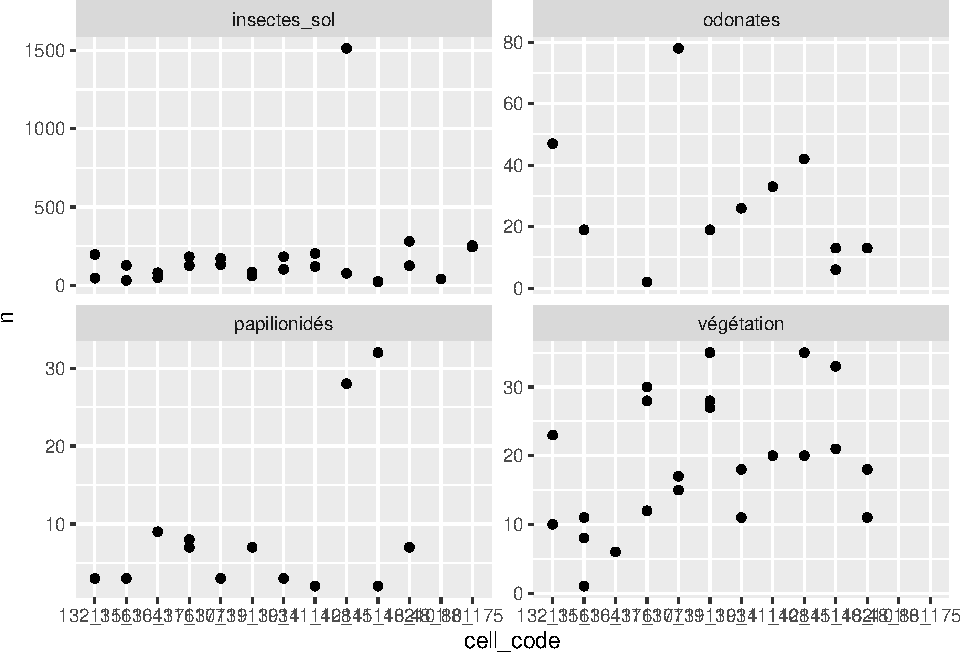
\includegraphics{indicators-bookdown_files/figure-latex/site_plot-1.pdf}

\bibliography{book.bib,packages.bib}


\end{document}
